% Apéndice - Modalidad Háptica

\chapter{Modalidad H\'{a}ptica} % Chapter title

\label{ch:mod_haptic} 

%----------------------------------------------------------------------------------------
% ### Introducción de capitulo
La modalidad háptica es la que permite la interacción con el órgano mas grande del cuerpo humano, la piel. Particularmente, el sentido del tacto. Este sentido, junto a la vista, permiten, por ejemplo, el rápido reconocimiento de escenarios, percibiendo profundidad y distancias estimadas con los elementos del ambiente así como también una referencia centrada en el usuario, \ie desde mi lugar donde están los elementos.
Una de las principales características del sentido del tacto, es que brinda una autopista directa al sistema nervioso, a través de su propio canal. Esto representa una ventaja con respecto a otros sentidos, como por ejemplo, vista y oído, ya que no requiere un procesamiento (reconocimiento de patrones) previo. Por otro lado, esto indica que la información obtenida por este canal es de mas bajo nivel o mas ``cruda'' y seguramente seran necesarias tareas de filtrado o adaptación de la entrada.



\section{Sentidos Involucrados}
El principal sentido afectado por esta modalidad es el del tacto. A través de este sentido, se pueden identificar dos interfaces, una cutánea y otra cinestésica. La primera se relaciona directamente con la piel y sus diferentes terminales sensitivas, la segunda, en cambio, con músculos y tendones y representa información sobre la ubicación espacial de todo nuestro cuerpo en el ambiente. Ambos canales proporcionan diferente \emph{feedback} al usuario y deberán ser capturados/sintetizados usando diferente hardware, \ie display táctil vs. display cinestésico. Ambos pueden trabajar en conjunto y a diferencia de otros sentidos, el tacto, permite una comunicación bidireccional entre usuario y sistema, de esta forma, se nota claramente que mediante el uso de este canal es posible aumentar claramente la experiencia de usuario, ya que se aumenta el \emph{feedback}. Una posible forma de distinguir estas interfaces, es en cuanto al caudal de información que intentemos enviar por el canal, \ie si solo necesitamos transmitir una alerta para corregir una acción vs. si deseamos transmitir información espacial al usuario; la primera puede ser solucionada usando la interfaz táctil y la segunda la cinestésica.

Existen diferentes formas de estimular el sentido del tacto, los receptores hápticos del cuerpo humano son de tres tipos: mecano-receptores (actúan de acuerdo a la fuerza o presión), termo-receptores (estimulados por la temperatura que reciben) y nociceptores (estimulados por el dolor).
Los sistemas mecano-receptores son los mas populares, y se pueden clasificar en cuatro diferentes sensaciones: presión, tacto, vibración y cosquilleo. La distribución de estos sensores no es uniforme en todo el cuerpo, por lo que aplicar una mecano-estimulación impactara de manera diferente de acuerdo al lugar de acción. Es una cuestión a tener en cuenta antes de desarrollar cualquier tipo de aplicación multimodal que planee utilizar este sentido. En el trabajo de \citet{hale2004deriving}, se clasifican y recomiendan distintas interfaces hápticas, siendo una guia importante al momento de desarrollar una interfaz que consuma esta modalidad.

\section{Interfaces Populares}
Algunas interfaces populares para esta modalidad son el dispositivo Falcon de \href{http://www.novint.com/index.php/novintfalcon}{Novint} o \href{http://www.dentsable.com/haptic-phantom-desktop.htm}{PHANTOM}, ambos de características similares, operan sobre la interfaz táctil brindando un punto de conocimiento al usuario, que mediante el uso del dispositivo puede enviar información aplicando presión y recibir un estimulo, mediante un sistema de motores de vibración. Dispositivos de este estilo, permiten reconocer texturas o ambientes a través de dicha estimulación viéndose limitados a un único punto de contacto, es decir no transmiten información masivamente a todo el cuerpo.

% FIGURA DE MODALIDAD HAPTICA
\begin{center}
  \begin{figure}[h]
    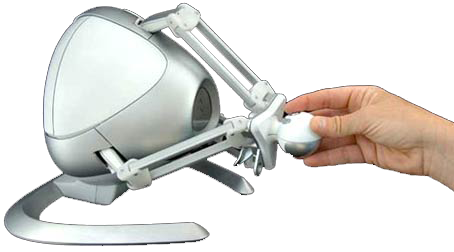
\includegraphics[scale=1,width=\textwidth]{gfx/novint1xe6}
    \caption{Dispositivo Falcon de la compañia Novint}
    \label{fig:apx_novint}
  \end{figure}
\end{center}

Es interesante destacar también la ocurrencia de estimuladores háptico es dispositivos de uso masivo como son los dispositivos móviles o smartphones y también, en los sistemas de entretenimiento, presentes en los joysticks, desde hace bastante tiempo. La interfaz con la que estos dispositivos interactúan es nuevamente la táctil, a través de un sistema de estímulos hacia el usuario, la intención común es brindar algún tipo de alerta sobre alguna acción a realizar.
La presencia de esta modalidad en dispositivos masivos fue una de las características que motivo a que sea una de las primeras modalidades en ser soportadas por la plataforma mediante el desarrollo de un driver.
Existen mas implementaciones de interfaces hápticas que las que se mencionan aquí, para mas información se recomienda ver el capitulo sobre la modalidad háptico de \citet{kortum2008hci}.

\section{Tecnología Utilizada}
En este trabajo se incluye un driver de modalidad que trabaja con displays táctiles y feedback vibro-táctil, por lo que se hará foco en la modalidad de trabajo de los mecano-receptores.
Para aprovechar la ocurrencia masiva de dispositivos vibro-táctiles e interfaces ''touch'', se decidió que el driver utilice el hardware incluido en los móviles, accediendo a los mismos a través de las interfaces estándar HTML5 correspondientes, \eg  \href{http://www.w3.org/TR/vibration/}{API de vibración}.
